% !TEX TS-program = pdflatex
% !TEX encoding = UTF-8 Unicode

% This is a simple template for a LaTeX document using the "article" class.
% See "book", "report", "letter" for other types of document.

\documentclass[11pt,titlepage]{article} % use larger type; default would be 10pt

\usepackage[utf8]{inputenc} % set input encoding (not needed with XeLaTeX)

%%% Examples of Article customizations
% These packages are optional, depending whether you want the features they provide.
% See the LaTeX Companion or other references for full information.

%%% PAGE DIMENSIONS
\usepackage{geometry} % to change the page dimensions
\geometry{a4paper} % or letterpaper (US) or a5paper or....
% \geometry{margin=2in} % for example, change the margins to 2 inches all round
% \geometry{landscape} % set up the page for landscape
%   read geometry.pdf for detailed page layout information

\usepackage{graphicx} % support the \includegraphics command and options
\usepackage{titlepic}

% \usepackage[parfill]{parskip} % Activate to begin paragraphs with an empty line rather than an indent

%%% PACKAGES
\usepackage{booktabs} % for much better looking tables
\usepackage{array} % for better arrays (eg matrices) in maths
\usepackage{paralist} % very flexible & customisable lists (eg. enumerate/itemize, etc.)
\usepackage{verbatim} % adds environment for commenting out blocks of text & for better verbatim
\usepackage{subfig} % make it possible to include more than one captioned figure/table in a single float
% These packages are all incorporated in the memoir class to one degree or another...

%%% HEADERS & FOOTERS
\usepackage{fancyhdr} % This should be set AFTER setting up the page geometry
\pagestyle{fancy} % options: empty , plain , fancy
\renewcommand{\headrulewidth}{0pt} % customise the layout...
\lhead{}\chead{}\rhead{}
\lfoot{}\cfoot{\thepage}\rfoot{}

%%% SECTION TITLE APPEARANCE
\usepackage{sectsty}
\allsectionsfont{\sffamily\mdseries\upshape} % (See the fntguide.pdf for font help)
% (This matches ConTeXt defaults)

%%% ToC (table of contents) APPEARANCE
\usepackage[nottoc,notlof,notlot]{tocbibind} % Put the bibliography in the ToC
\usepackage[titles,subfigure]{tocloft} % Alter the style of the Table of Contents
\renewcommand{\cftsecfont}{\rmfamily\mdseries\upshape}
\renewcommand{\cftsecpagefont}{\rmfamily\mdseries\upshape} % No bold!

\newenvironment{changemargin}[3]{%
\begin{list}{}{%
\setlength{\topsep}{0pt}%
\setlength{\headsep}{#3}%
\setlength{\leftmargin}{#1}%
\setlength{\rightmargin}{#2}%
\setlength{\listparindent}{\parindent}%
\setlength{\itemindent}{\parindent}%
\setlength{\parsep}{\parskip}%
}%
\item[]}{\end{list}}

%Table Formatting
\usepackage{tabularx,hhline}
\usepackage{pbox}
\usepackage{booktabs}
\usepackage{makecell}
\usepackage{float}

%%% END Article customizations

%%% The "real" document content comes below...

\titlepic{
\includegraphics[scale=0.60]{polimi_logo.jpg}}
\title{Project Plan Document \\ \vspace{1cm} \large{Version 1.0}}
\author{Giorgio Pea(Mat. 853872), Andrea Sessa(Mat. 850082)}
\date{2/2/2016}

\begin{document}

\maketitle

\newpage

\tableofcontents

\newpage

\section{Introduction}
  \subsection{Purpose}
    The main purpose of this document is to analyze effort and cost for MyTaxiService.
    The analysis is performed using two different models:
    \begin{itemize}
     \item Function Points: to determine the size and the overall complexity of the project
     \item COCOMO II: to determine the effort and cost of the project
    \end{itemize}
    In the final part of the document are also included a Gantt diagram to visualize the page
    general schedule of the project and a resource allocation diagram to show how the team 
    members have been assigned to the various tasks.

  \subsection{Acronyms}
    \begin{itemize}
     \item \textbf{RASD:} Requirements Analysis and Specification Document
     \item \textbf{DD:} Design Document
     \item \textbf{ITPD:} Integration Test Plan Document
     \item \textbf{AWT:} Approximate Waiting Time
    \end{itemize}
  \subsection{References}
    \begin{itemize}
     \item COCOMO II Specification
     \item Function Point Specification
    \end{itemize}

\section{Function Point Analysis}
  \subsection{Introduction}
    The function point analysis is a technique that provides an algorithmic and statistical estimation of the size of a software project.\newline
    This estimation is based on the following elements of the product model:
    \begin{itemize}
     \item \textbf{Internal Logic Files:} It represents a homogeneous set of data managed and created by the application
     \item \textbf{External Logic Files:} It represents a homogeneous set of data used by the application but generated and maintained by other applications
     \item \textbf{External Input:} It represents a set of elementary procedures to elaborate data coming from the external environment
     \item \textbf{External Output:} It represents a set of procedures that generate data for the external environment with a significant elaboration of logic files
     \item \textbf{External Inquiry:} It represents a set of input/output operations that do not require a significant elaboration of logic files
    \end{itemize}
    The following table shows the coefficients to be used in the UFP computations and relative to the different function types and their estimated complexity:\newline
    \begin{center}
      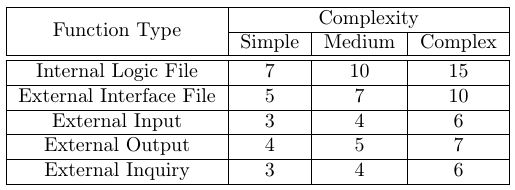
\includegraphics[scale=0.5]{fptable.png}
    \end{center}

  \subsection{Internal Logic Files}
     The system needs to store information about: \newline \newline
     \textbf{User}\newline
     This data entity consist in a small set of information, for this reason its complexity has been considered \textbf{SIMPLE}\newline\newline
     \textbf{Administrator}\newline
     This data entity consist in a small set of information, for this reason its complexity has been considered \textbf{SIMPLE}\newline\newline
     \textbf{Mtaxi driver}\newline
     This data entity consist in a small set of information, for this reason its complexity has been considered \textbf{SIMPLE}\newline\newline
     \noindent \textbf{Mtaxi}\newline
     This data entity consist in a small set of information, for this reason its complexity has been considered \textbf{SIMPLE}\newline\newline
     \textbf{Work Time Table}\newline
     This data entity consist in a small set of information, for this reason its complexity has been considered \textbf{SIMPLE}\newline\newline
     \textbf{Zone}\newline
     This data entity consist in a small set of information, for this reason its complexity has been considered \textbf{SIMPLE}\newline\newline
     \textbf{Location}\newline
     This data entity consist in a small set of information, for this reason its complexity has been considered \textbf{SIMPLE}\newline\newline
     \textbf{Ride Request} 
     This data entity consist in a small set of information, for this reason its complexity has been considered \textbf{SIMPLE}\newline\newline
     \textbf{Booking Request}
     This data entity consist in a small set of information, for this reason its complexity has been considered \textbf{SIMPLE}\newline\newline
     \textbf{Queue}
     This data entity consist in a small set of information, for this reason its complexity has been considered \textbf{SIMPLE}\newline
     
     \begin{center}
      $ ILF Function Points = numberOfILF * 7 = 7 * 7 = 49 $
     \end{center}

   \subsection{External Logic Files}
    The system needs to access data about:\newline\newline
    \textbf{External Traffic data}\newline
    The structure of this data could be complex and could need a digest process, for this reason its complexity has been considered \textbf{MEDIUM}\newline
    
    \begin{center}
     $ ILF Function Points = numberOfELF * 7 = 1 * 7 = 7 $
    \end{center}
    
    \subsection{External Input}
     The system needs to process the following input: \newline

      \noindent \textbf{Ride Request creation}\newline
      This operation requires the user to perform few and simple actions and the system to perform straightforward checks and data procedures,
      for this reason its complexity has been considered \textbf{SIMPLE}\newline\newline
      
      \noindent \textbf{Booking Request creation}\newline
      This operation requires the user to perform few and simple actions and the system to perform straightforward checks and data procedures,
      for this reason its complexity has been considered \textbf{SIMPLE}\newline\newline
      
      \noindent \textbf{Booking Request editing}\newline
      This operation requires the user to perform few and simple actions and the system to perform straightforward checks and data procedures,
      for this reason its complexity has been considered \textbf{SIMPLE}\newline\newline
      
      \noindent \textbf{User Login/Logout}\newline
      This operation requires the user to perform few and simple actions and the system to perform straightforward checks and data procedures,
      for this reason its complexity has been considered \textbf{SIMPLE}\newline\newline
      
      \noindent \textbf{User Registration}\newline
      This operation requires the user to perform few and simple actions and the system to perform straightforward checks and data procedures,
      for this reason its complexity has been considered \textbf{SIMPLE}\newline\newline
      
      \noindent \textbf{Mtaxi Driver Registration}\newline
      This operation requires the Mtaxi driver to perform few and simple actions and the system to perform straightforward checks and data procedures,
      for this reason its complexity has been considered \textbf{SIMPLE}\newline\newline
      
      \noindent \textbf{Driver Notification}\newline
      This operation requires the user to perform few and simple actions and the system(including the MYT device) more complex and numerous procedures,
      for this reason its complexity has been considered \textbf{MEDIUM}\newline\newline
      
      \noindent \textbf{Administrator Operations}\newline
      This operation requires the administrator to perform few and simple actions and the system to perform straightforward checks and data procedures,
      for this reason its complexity has been considered \textbf{SIMPLE}\newline
      
      \begin{center}
	$ EI Function Points = numberOfSimpleEI * 3 + numberOfMediumEI * 4 = 7 * 3 + 1 * 4 = 25 $
      \end{center}
    
    \subsection{External Output}
      \textbf{AWT Notification}\newline
      This operation requires the system to perform complex calculations on traffic data and Mtaxi positions, for this reason its complexity has been considered \textbf{COMPLEX}\newline\newline

      
      
      \noindent \textbf{Zone Change Notification}\newline
      This operation implies that the system noticed an unbalanced distribution of Mtaxi in city zones; this last process requires complex and numerous
      calculations and data checks, this operation requires the system to perform complex calculations on traffic data and Mtaxi positions, for this reason its complexity has been considered \textbf{COMPLEX}\newline
      \begin{center}
	$ EO Function Points = numberOfEO * 7 = 2 * 7 = 14 $
      \end{center}
      
    \subsection{External Inquiry}
       \textbf{User Profile Visualization}\newline
       This operation requires the system to retrieve and elaborate data in a simple way, for this reason its complexity has been considered \textbf{SIMPLE}\newline\newline
       \textbf{User Ride Request Visualization}\newline
       This operation requires the system to retrieve and elaborate data in a simple way, for this reason its complexity has been considered \textbf{SIMPLE}\newline\newline
       \textbf{User Booking Request Visualization}\newline
       This operation requires the system to retrieve and elaborate data in a simple way, for this reason its complexity has been considered \textbf{SIMPLE}\newline\newline
       \textbf{Mtaxi Notification Visualization}\newline
       This operation requires the system to retrieve and elaborate data in a simple way, for this reason its complexity has been considered \textbf{SIMPLE}\newline\newline
       \textbf{Mtaxi Accident Reports Visualization}\newline
       This operation requires the system to retrieve and elaborate data in a simple way, for this reason its complexity has been considered \textbf{SIMPLE}\newline\newline
       \textbf{Mtaxi Bad Behavior Reports Visualization}\newline
       This operation requires the system to retrieve and elaborate data in a simple way, for this reason its complexity has been considered \textbf{SIMPLE}\newline
       \begin{center}
	$ EI Function Points = numberOfEI * 3 = 6 * 3 = 18 $
       \end{center}
     
     \subsection{Summary}
	\begin{center}
	$ Total Function Points(UFP) = 49 + 7 + 25 + 14 + 18  = 113 $
	\end{center}

\newpage
\section{COCOMO II Analysis}
  \subsection{Introduction}
    COCOMO II is algorithmic and statistical methodology used to estimate the effort of a software project.
    This estimation requires, as input data, the project size(SLOCs) and the project's scale and cost drivers coefficients.\newline
    
    \begin{itemize}
     \item \textbf{Cost Drivers:} COCOMO II has 17 cost drivers, which represent factors that contribute in significant way to the effort required to complete the software project
     \item \textbf{Scale Drivers:} COCOMO II has 5 scale driver which represent process specific factors that contribute in significant way to the effort required to complete the software project
    \end{itemize}
    
    In this case the previous Function Points analysis is used to estimate the SLOC number.\newline
    Assuming that the programming language used for the will be Java EE, the conversion factor between the 
    total function point counts(UFP) and the SLOC is 46.
    \begin{equation}
     SLOCs = conversionFactor * UFP = 113 * 46 = 5198
    \end{equation}

    The COCOMO II methodology estimates the effort needed to complete a software project via following equation:
    \begin{equation}
     effort = 2.94 * EAF * (KSLOC)^E
    \end{equation}
    where EAF(Effort Adjustment Factor) depends on the Cost Drivers and E is derived from the Scale Drivers.\newline
    COCOMO II estimates also the duration of a software project via following equation:
    \begin{equation}
     duration = 3.67 * (effort)^E
    \end{equation}
  \newpage
  \subsection{Analysis}
    In this section is included the final COCOMO analysis performed using a tool available at:\newline
    http://csse.usc.edu/tools/COCOMOII.php\newline
    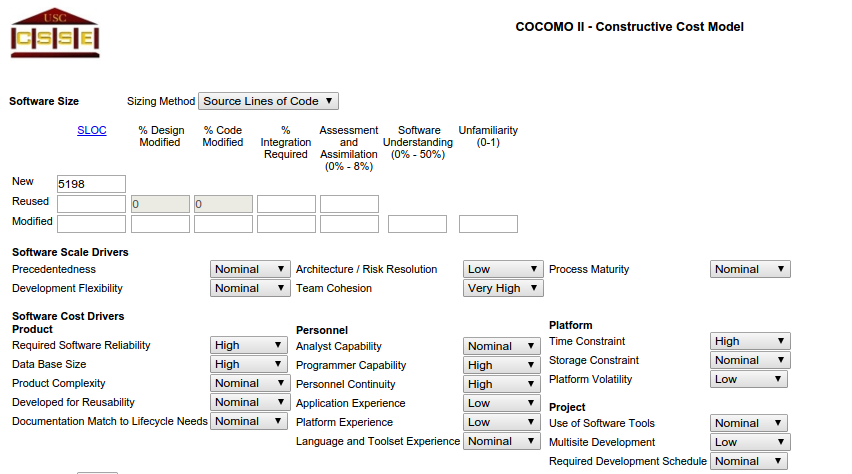
\includegraphics[scale=0.5]{cocomo1.png}
    \newpage
    \begin{center}
      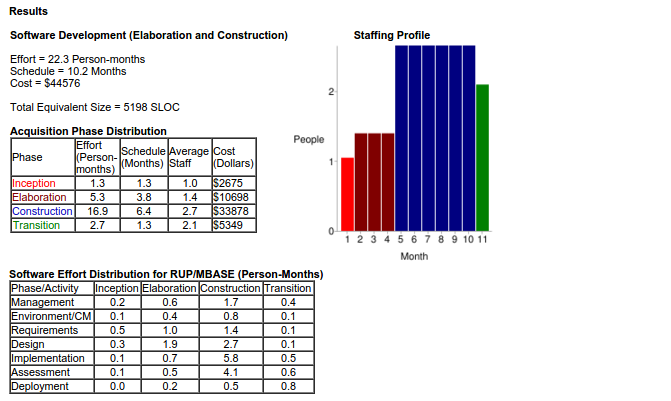
\includegraphics[scale=0.6]{cocomo2.png}
    \end{center}

\newpage

\section{Task Gantt Diagram}
 In this section is included a gantt diagram that represents the tasks in which the project is divided.\newline
 Slashed tasks are not represented in scale with respect to the others activities due to space constraints.\newline 
 \begin{center}
  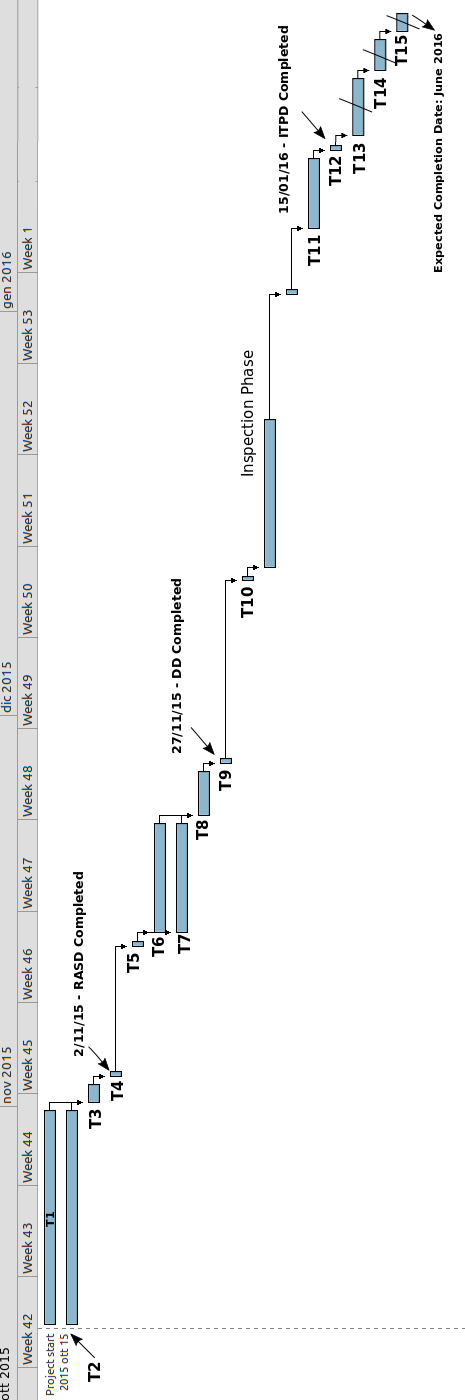
\includegraphics[scale=0.35]{ganttnew.png}
 \end{center}
\newpage

\noindent In the following paragraph is included an explanation of each task and of its duration in terms of work hours
\begin{itemize}
 \item \textbf{T1:} Requirements Specification - Duration: 29h
 \item \textbf{T2:} RASD Diagrams Specification - Duration: 29h
 \item \textbf{T3:} Alloy Model Definition - Duration: 4h
 \item \textbf{T4:} RASD Revision - Duration: 2h
 \item \textbf{T5:} RASD Post-Presentation Revision - Duration: 2h
 \item \textbf{T6:} Architecture Specification - Duration: 18h
 \item \textbf{T7:} DD Diagrams Specification - Duration: 18h
 \item \textbf{T8:} Algorithms Definition - Duration: 2h
 \item \textbf{T9:} DD Revision - Duration: 2h
 \item \textbf{T10} DD Post-Presentation Revision - Duration: 2h
 \item \textbf{T11:} Integration Test Plan Definition - Duration: 8h
 \item \textbf{T12:} ITPD Revision: Duration: 1h
\end{itemize}
 For the following tasks we assume that the implementation phase is divided into two main development activities(Backend and Frontend implementation).
 The duration of the development phase is estimated both on the base of the COCOMO analysis and on our previous experience with others projects.\newline
\begin{itemize}
 \item \textbf{T13:} Backend implementation - Duration: 2 months
 \item \textbf{T14:} Frontend implementation - Duration: 1.5 months
 \item \textbf{T15:} Acceptance Testing - Duration: 0.5 months
\end{itemize}

 

\newpage
\section{Resource Allocation Diagram}
  In this section are included two diagrams showing how the two team members(Andrea Sessa, Giorgio Pea) have been allocated to the tasks
  described in the previous section.\newline
  The work time is indicated in gray while the free time is indicated in green.
  For each activity its allocated time is indicated in percentage with respect to the total amount of time available for the set of activities this one belongs to.\newline
  Due to space constraints the diagrams are shown in the next two pages.\newline
  \newpage
  \textbf{Allocation Diagram: Andrea Sessa}\newline
  \begin{center}
       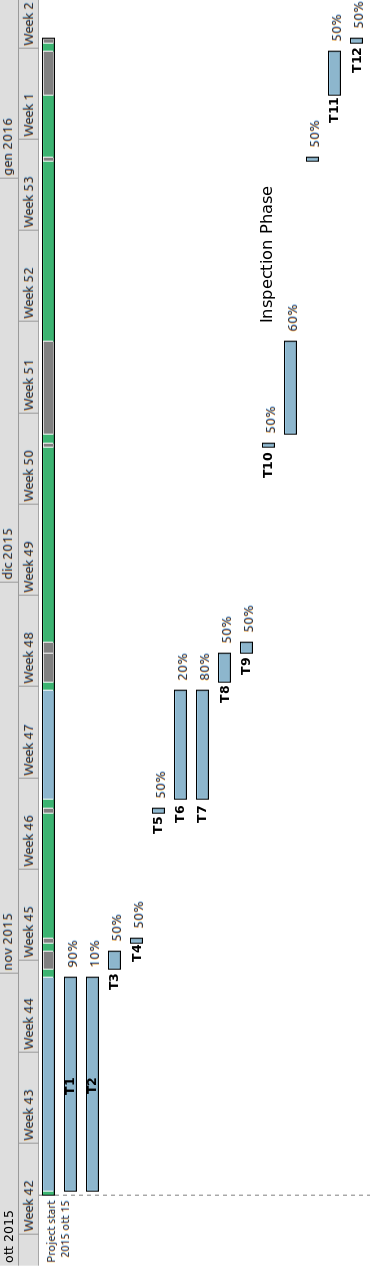
\includegraphics[scale=0.35]{res1.png}
  \end{center}
  \newpage
  \textbf{Allocation Diagram: Giorgio Pea}\newline
  \begin{center}
       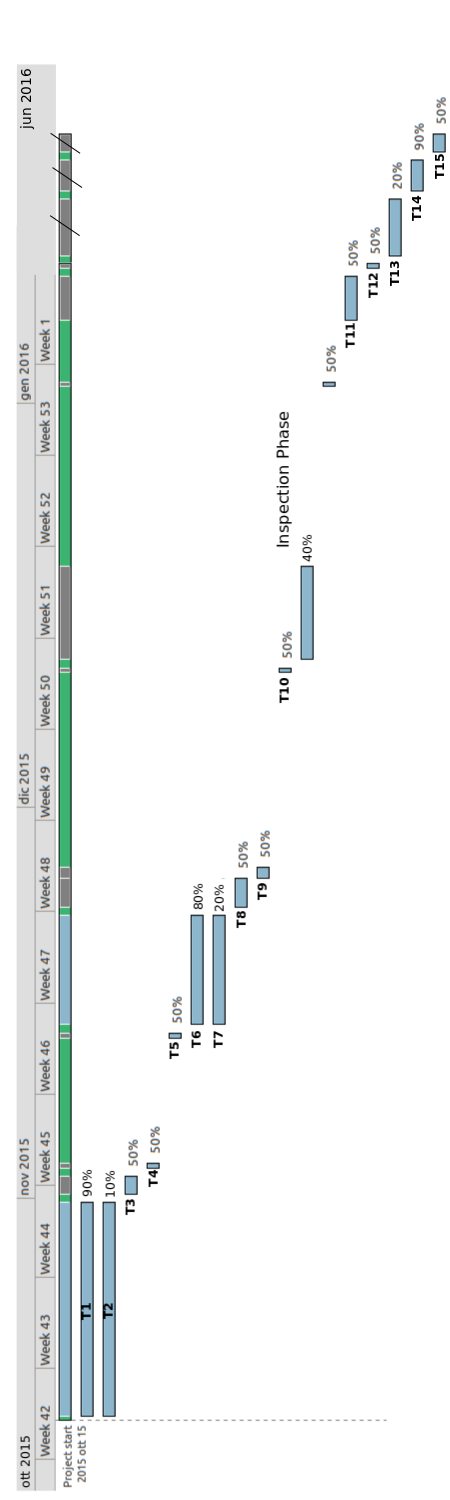
\includegraphics[scale=0.35]{res2.png}
  \end{center}

\newpage
\section{Risks Detection and Management}
In this section is included a list of possible risks that can occur during the project.\newline

\subsection{Process Risks}
  \begin{enumerate}
   \item Key development figures may be ill at critical times during the project\newline
	 \textbf{Probability:} Moderate\newline
	 \textbf{Effect:} Serious\newline
	 \textbf{Recovery Strategy:} Reorganize the team so that there is more overlap of work and people therefore understand each other’s jobs\newline
  \item Important changes to the project's requirements and design may occur.
	 \textbf{Probability:} Low\newline
	 \textbf{Effect:} Critical\newline
	 \textbf{Recover Strategy:} Use previously derived traceability information to assess requirements the impact of the requirements' change\newline
  \item Key development figures may be busy at critical times during the project\newline
	\textbf{Probability:} Moderate\newline
	\textbf{Effect:} Serious\newline
	\textbf{Recover Strategy: } Reorganize the resource allocation plan to match the availability of the staff with the project schedule
  \item Underestimated development time\newline
    \textbf{Probability:} Moderate\newline
    \textbf{Effect:} Serious\newline
    \textbf{Recover Strategy:} Investigate the possibility of using COTS or try to renegotiate the deadlines.\newline
  \end{enumerate}

\subsection{Technical Risks}
  \begin{enumerate}
   \item Database or other key components in the architecture do not perform as expected\newline
    \textbf{Probability:} Low\newline
    \textbf{Effect:} Serious\newline
    \textbf{Recover Strategy:} Investigate the possibility of buying a higher-performance components.\newline
   \item The architecture proposed for the project cannot be implemented due to economical or other reasons\newline
    \textbf{Probability:} Moderate\newline
    \textbf{Effect:} Serious\newline
    \textbf{Recover Strategy:} Investigate the possibility of finding a feasible architecture that can be as much compatible as possible with the previous one.\newline
  \end{enumerate}

\subsection{Business Risks}
  We assume for this section that we are developing MyTaxiService for a real-world company.\newline
  \begin{enumerate}
   \item The organization is restructured, so that its to management changes\newline
    \textbf{Probability:} Low\newline
    \textbf{Effect:} Serious\newline
    \textbf{Recover Strategy:} Prepare a briefing document for the top management showing how the project is making a very important contribution to the goals of the business.\newline
   \item The organization find itself in serious financial problems\newline
    \textbf{Probability:} Low/Moderate\newline
    \textbf{Effect:} Catastrophic\newline
    \textbf{Recover Strategy:} Prepare a briefing document for the management showing how the project goals are fundamental for the company's business \newline
  \end{enumerate}

\newpage

\section{Appendix}
  	\subsection{Tools}
		\begin{itemize}
			\item \textbf{Planner:} to draw gantt and resource diagrams
			\item \LaTeX \textbf{/ Atom:} to redact this document
		\end{itemize}

	\subsection{Hours}
		\begin{itemize}
			\item Andrea Sessa: 12 hours
			\item Giorgio Pea: 8 hours
		\end{itemize}

\end{document}
